% ============================================================
%  THGNN Presentation — Financial Time Series Forecasting
%  Beamer / metropolis theme
% ============================================================
\documentclass[aspectratio=169, 10pt]{beamer}

% ---- Theme --------------------------------------------------
\usetheme{metropolis}
\usepackage{appendixnumberbeamer}

% ---- Packages -----------------------------------------------
\usepackage{booktabs}
\usepackage{amsmath, amssymb}
\usepackage{mathtools}
\usepackage{graphicx}
\usepackage{xcolor}
\usepackage{tikz}
\usetikzlibrary{shapes.geometric, arrows.meta, positioning, fit, backgrounds, calc}
\usepackage{pgfplots}
\pgfplotsset{compat=1.18}
\usepackage{hyperref}
\usepackage{algorithm}
\usepackage{algpseudocode}
\usepackage{multirow}
\usepackage{array}
\usepackage{colortbl}

% ---- Colour palette -----------------------------------------
\definecolor{primary}{HTML}{1B4F72}
\definecolor{accent}{HTML}{2E86C1}
\definecolor{positive}{HTML}{1E8449}
\definecolor{negative}{HTML}{C0392B}
\definecolor{neutral}{HTML}{7F8C8D}
\definecolor{highlight}{HTML}{F39C12}
\definecolor{lightbg}{HTML}{EBF5FB}
\definecolor{darkbg}{HTML}{1A252F}

\setbeamercolor{frametitle}{bg=primary, fg=white}
\setbeamercolor{progress bar}{fg=accent}
\setbeamercolor{alerted text}{fg=highlight}
\setbeamercolor{block title}{bg=accent, fg=white}
\setbeamercolor{block body}{bg=lightbg}

% ---- Metadata -----------------------------------------------
\title{Financial Time Series Forecasting\\with Graph Neural Networks}
\subtitle{THGNN: Temporal and Heterogeneous GNN for Nifty 50 Stock Prediction}
\author{Debarshi Chakraborty}
\date{\today}
\institute{Financial Time Series Forecasting Project}

% ---- Custom commands ----------------------------------------
\newcommand{\pos}{\textcolor{positive}{\textbf{+}}}
\newcommand{\neg}{\textcolor{negative}{\textbf{--}}}
\newcommand{\myvec}[1]{\mathbf{#1}}
\newcommand{\todo}[1]{\textcolor{red}{\textbf{[#1]}}}

% ============================================================
\begin{document}

\maketitle

% ---- Table of Contents --------------------------------------
\begin{frame}{Outline}
  \setbeamertemplate{section in toc}[sections numbered]
  \tableofcontents[hideallsubsections]
\end{frame}

% ============================================================
\section{Motivation \& Problem Statement}
% ============================================================

\begin{frame}{The Stock Ranking Problem}
  \begin{columns}[T]
    \begin{column}{0.55\textwidth}
      \textbf{Goal:} Given $N$ stocks observed over $T$ days, predict their
      \emph{relative cross-sectional ranking} at $t{+}1$.

      \bigskip
      \textbf{Key challenges:}
      \begin{itemize}
        \item Market is non-stationary and noisy
        \item Stocks are \alert{not independent} — sector shocks, macro events
        \item Relationships are \alert{dynamic}: correlations change over time
        \item Pure regression (MSE) does not align with portfolio objectives
      \end{itemize}

      \bigskip
      \textbf{Evaluation metric:} Information Coefficient (IC) \\
      \quad $= \text{Spearman}(\hat{r},\, r)$\\
      \quad IC $> 0.05$ is practically useful;\; IC $> 0.10$ is strong.
    \end{column}
    \begin{column}{0.42\textwidth}
      \begin{block}{Task Definition}
        \textbf{Input:} $\myvec{X} \in \mathbb{R}^{N \times T \times F}$\\
        \quad $N=50$ stocks (Nifty 50)\\
        \quad $T=20$ trading days look-back\\
        \quad $F=6$ features (OHLCV + turnover)
        \bigskip\\
        \textbf{Output:} $\hat{\myvec{r}} \in \mathbb{R}^{N}$\\
        \quad Predicted next-day return per stock
        \bigskip\\
        \textbf{Objective:}\\
        \quad $\max\;\text{Spearman}(\hat{\myvec{r}},\, \myvec{r}_{t+1})$
      \end{block}
    \end{column}
  \end{columns}
\end{frame}

\begin{frame}{Why Graph Neural Networks?}
  \begin{center}
  \begin{tikzpicture}[
    node distance=2.2cm,
    stock/.style={circle, draw=accent, fill=lightbg, minimum size=0.9cm, font=\small\bfseries},
    posedge/.style={-Latex, thick, positive, bend left=20},
    negedge/.style={-Latex, thick, negative, bend right=20, dashed},
    label/.style={font=\footnotesize, text=neutral}
  ]
    \node[stock] (REL) {REL};
    \node[stock, right=of REL] (TCS) {TCS};
    \node[stock, below=of REL] (HDFC) {HDFC};
    \node[stock, below=of TCS] (INFY) {INFY};
    \node[stock, right=of TCS] (ITC) {ITC};

    \draw[posedge] (REL) to node[above, label]{$\rho=0.62$} (TCS);
    \draw[posedge] (TCS) to node[right, label]{$\rho=0.71$} (INFY);
    \draw[posedge] (HDFC) to node[below, label]{$\rho=0.55$} (INFY);
    \draw[negedge] (REL) to node[left, label]{$\rho=-0.38$} (HDFC);
    \draw[negedge] (ITC) to node[above, label]{$\rho=-0.42$} (INFY);

    \node[below=0.2cm of HDFC, label, align=center]
      {\textcolor{positive}{$\longrightarrow$ Positive corr. (moves together)}};
    \node[above=0.1cm of REL, xshift=3.5cm, label, align=center]
      {\textcolor{negative}{$--\to$ Negative corr. (moves inversely)}};
  \end{tikzpicture}
  \end{center}
  \vspace{-0.3cm}
  \begin{block}{}
    A graph representation allows the model to \textbf{propagate information}
    across correlated stocks — a fundamental advantage over treating each stock
    independently.
  \end{block}
\end{frame}

% ============================================================
\section{Literature Review \& Model Evolution}
% ============================================================

\begin{frame}{Evolution of Stock Prediction Architectures}
  \begin{tikzpicture}[
    node distance=0.5cm and 1.2cm,
    box/.style={rounded corners, draw, minimum width=3.2cm, minimum height=1.2cm,
                align=center, font=\small},
    arrow/.style={-Latex, thick, accent},
    stage/.style={font=\footnotesize\itshape, text=neutral}
  ]
    \node[box, fill=lightbg, draw=neutral] (master)
      {\textbf{MASTER} \\ \scriptsize Market-guided \\ attention gating};

    \node[box, fill=lightbg, draw=neutral, below=0.6cm of master] (stockmixer)
      {\textbf{StockMixer} \\ \scriptsize Patch-based \\ indicator mixing};

    \node[box, fill=accent!20, draw=accent, right=1.5cm of master, yshift=-0.6cm] (thgnn)
      {\textbf{THGNN} \\ \scriptsize Heterogeneous \\ dynamic graph};

    \node[box, fill=positive!15, draw=positive, right=1.5cm of thgnn] (hyper)
      {\textbf{Hypergraph} \\ \scriptsize STHAN-SR \\ MaGNet};

    \draw[arrow] (master) -- node[above, stage, xshift=-0.3cm]{relational\,gap} (thgnn);
    \draw[arrow] (stockmixer) -- (thgnn);
    \draw[arrow] (thgnn) -- node[above, stage]{pairwise\,limit} (hyper);

    % Limitation labels
    \node[below=0.15cm of master, font=\scriptsize, text=negative, align=center]
      {Static / no \\ inter-stock graph};
    \node[below=0.15cm of stockmixer, font=\scriptsize, text=negative, align=center]
      {Independent stock \\ representations};
    \node[below=0.15cm of thgnn, font=\scriptsize, text=negative, align=center]
      {Pairwise edges only;\\ no group dynamics};
    \node[below=0.15cm of hyper, font=\scriptsize, text=positive, align=center]
      {Higher-order \\ hyperedges};
  \end{tikzpicture}

  \vspace{0.4cm}
  This work implements \alert{THGNN}, the first step towards relational
  stock modelling, and analyses the path toward hypergraph architectures.
\end{frame}

\begin{frame}{MASTER \& StockMixer — Strengths and Gaps}
  \begin{columns}[T]
    \begin{column}{0.48\textwidth}
      \textbf{MASTER}
      \begin{itemize}
        \item Market-index signal gates each stock's temporal features
        \item Sophisticated temporal attention for intra-stock dynamics
        \item[\textcolor{negative}{\faTimesCircle}] \textcolor{negative}{Static or no inter-stock graph}
        \item[\textcolor{negative}{\faTimesCircle}] \textcolor{negative}{Homogeneous relationship treatment}
      \end{itemize}
      \bigskip
      \textbf{StockMixer}
      \begin{itemize}
        \item Patch-based temporal encoding captures multi-scale trends
        \item Indicator mixing across feature channels
        \item[\textcolor{negative}{\faTimesCircle}] \textcolor{negative}{Stocks remain independent}
        \item[\textcolor{negative}{\faTimesCircle}] \textcolor{negative}{No relational information flow}
      \end{itemize}
    \end{column}
    \begin{column}{0.48\textwidth}
      \begin{alertblock}{Core Gap Addressed by THGNN}
        Both models process each stock's signals \emph{in isolation}.
        Real markets exhibit strong cross-stock dependencies that cannot
        be captured without explicit graph structure.
      \end{alertblock}
      \bigskip
      \textbf{THGNN's answers:}
      \begin{enumerate}
        \item Day-specific correlation graph (dynamic, not static)
        \item Separate \textcolor{positive}{positive} and \textcolor{negative}{negative}
              GAT heads (heterogeneous, not homogeneous)
        \item Semantic attention over self vs.\ neighbour channels
      \end{enumerate}
    \end{column}
  \end{columns}
\end{frame}

\begin{frame}{Beyond THGNN — The Hypergraph Frontier}
  \begin{columns}[T]
    \begin{column}{0.48\textwidth}
      \textbf{Standard GNN limitation (THGNN):}
      \begin{itemize}
        \item Edges are \emph{pairwise} only: $e = (u, v)$
        \item Cannot natively represent group shocks\\
              (e.g.\ an entire sector reacting to one event)
        \item Decomposing groups into pairs loses higher-order signal
      \end{itemize}
      \bigskip
      \textbf{Hypergraph solution:}
      \begin{itemize}
        \item \textbf{Hyperedge} $e \subseteq V$: connects any subset of stocks
        \item MaGNet: probabilistic hyperedges —
              stocks have \emph{soft membership} across market themes
        \item STHAN-SR: reformulates prediction as
              \emph{learning-to-rank} for direct profit optimisation
      \end{itemize}
    \end{column}
    \begin{column}{0.48\textwidth}
      \begin{tikzpicture}[scale=0.88]
        % Standard graph
        \node[font=\small\bfseries, text=neutral] at (1.2, 3.0) {Standard Graph};
        \foreach \x/\lbl in {0/A, 1.2/B, 2.4/C, 1.2/D}{
          \node[circle, draw=accent, fill=lightbg, minimum size=0.7cm,
                font=\scriptsize] (\lbl) at (\x, \ifnum\x<2 2.2 \else 2.2 \fi)
                {\lbl};
        }
        \node[circle, draw=accent, fill=lightbg, minimum size=0.7cm,
              font=\scriptsize] (D) at (1.2, 1.2) {D};
        \draw[accent] (A)--(B) (B)--(C) (A)--(D) (B)--(D);

        % Hypergraph
        \node[font=\small\bfseries, text=neutral] at (5.2, 3.0) {Hypergraph};
        \foreach \x/\lbl in {3.8/E, 5.0/F, 6.2/G}{
          \node[circle, draw=positive, fill=positive!10, minimum size=0.7cm,
                font=\scriptsize] (\lbl) at (\x, 2.2) {\lbl};
        }
        \node[circle, draw=positive, fill=positive!10, minimum size=0.7cm,
              font=\scriptsize] (H) at (5.0, 1.2) {H};
        \begin{scope}[on background layer]
          \node[draw=positive, fill=positive!15, ellipse, fit=(E)(F)(G),
                inner sep=4pt, opacity=0.6] {};
          \node[draw=highlight, fill=highlight!15, ellipse, fit=(F)(G)(H),
                inner sep=4pt, opacity=0.6] {};
        \end{scope}
        \node[font=\scriptsize, text=positive] at (5.0, 2.85) {sector A};
        \node[font=\scriptsize, text=highlight] at (5.9, 1.0) {sector B};
      \end{tikzpicture}
    \end{column}
  \end{columns}
\end{frame}

% ============================================================
\section{THGNN Architecture}
% ============================================================

\begin{frame}{THGNN — End-to-End Architecture Overview}
  \begin{tikzpicture}[
    scale=0.9, every node/.style={font=\scriptsize},
    block/.style={draw, rounded corners, minimum width=2.4cm, minimum height=0.75cm,
                  align=center, fill=lightbg},
    arrow/.style={-Latex, thick, accent},
    label/.style={font=\tiny, text=neutral, align=center}
  ]
    \node[block, fill=darkbg, text=white] (input) at (0,0)
      {Input\\$\mathbf{X}: (N,20,6)$};

    \node[block] (norm) at (2.4,0) {LayerNorm\\+ CS Demean};
    \node[block, fill=accent!25] (gru) at (4.8,0) {GRU\\$\mathbf{h}_T:(N,128)$};

    \node[block, fill=positive!20] (posgat) at (7.2, 0.6)
      {Pos-GAT\\$\rho > \theta$};
    \node[block, fill=negative!15] (neggat) at (7.2,-0.6)
      {Neg-GAT\\$\rho < -\theta$};
    \node[block] (self) at (7.2, 0) {Self\\MLP};

    \node[block, fill=highlight!25] (semat) at (9.8, 0)
      {Semantic\\Attention};

    \node[block] (pn) at (11.9, 0) {PairNorm\\PN-SI};
    \node[block, fill=darkbg, text=white] (pred) at (13.9, 0)
      {Linear\\$(N,1)$};

    \draw[arrow] (input) -- (norm);
    \draw[arrow] (norm) -- (gru);
    \draw[arrow] (gru.east) -- ++(0.2,0) |- (posgat.west);
    \draw[arrow] (gru.east) -- ++(0.2,0) -- (self.west);
    \draw[arrow] (gru.east) -- ++(0.2,0) |- (neggat.west);
    \draw[arrow] (posgat.east) -| (semat.north);
    \draw[arrow] (self.east) -- (semat.west);
    \draw[arrow] (neggat.east) -| (semat.south);
    \draw[arrow] (semat) -- (pn);
    \draw[arrow] (pn) -- (pred);

    % adjacency inputs
    \node[label, text=positive] at (7.2, 1.35) {pos\_adj};
    \node[label, text=negative] at (7.2,-1.35) {neg\_adj};

    % Stage labels
    \foreach \x/\txt in {1.2/\textbf{(1) Norm}, 3.6/\textbf{(2) Temporal},
                          7.2/\textbf{(3) Spatial}, 9.8/\textbf{(4) Semantic},
                          12.9/\textbf{(5) Output}} {
      \node[label, text=accent] at (\x,-1.3) {\txt};
    }
  \end{tikzpicture}

  \vspace{0.2cm}
  \begin{columns}[T]
    \begin{column}{0.48\textwidth}
      \small
      Each forward pass processes \textbf{one trading day} as a graph of
      50 stock nodes.
    \end{column}
    \begin{column}{0.48\textwidth}
      \small
      Output: a scalar \emph{predicted return} per stock, used to rank
      the full universe.
    \end{column}
  \end{columns}
\end{frame}

\begin{frame}{Stage 1 \& 2 — Normalisation and Temporal Encoding}
  \begin{columns}[T]
    \begin{column}{0.48\textwidth}
      \textbf{Input Normalisation}

      \begin{block}{LayerNorm per timestep}
        \vspace{-0.3em}
        \[
          \tilde{x}_{i,t} = \text{LayerNorm}_F(x_{i,t})
        \]
      \end{block}
      Prevents volume/turnover ($\times 100$) from dominating GRU gates.

      \vspace{0.3cm}
      \textbf{Cross-sectional demeaning:}
      \[
        x_{i,t} \leftarrow x_{i,t} - \frac{1}{N}\sum_{j=1}^N x_{j,t}
      \]
      Removes market-wide beta; model focuses on \emph{relative} stock behaviour.
    \end{column}
    \begin{column}{0.48\textwidth}
      \textbf{GRU Temporal Encoder}

      \begin{block}{GRU configuration}
        \vspace{-0.3em}
        \begin{align*}
          &\text{input\_size} = 6,\quad \text{hidden} = 128\\
          &\text{num\_layers} = 1,\quad \text{dropout} = 0.3
        \end{align*}
      \end{block}

      Each stock's 20-day sequence is encoded \emph{independently}:
      \[
        \myvec{h}_{i,T} = \text{GRU}(\myvec{x}_{i,1:T})
        \;\in\; \mathbb{R}^{128}
      \]
      Only final hidden state $h_T$ is kept — encodes the full temporal
      context in a fixed-size vector.
    \end{column}
  \end{columns}
\end{frame}

\begin{frame}{Stage 3 — Heterogeneous Graph Attention (GAT)}
  \textbf{Two separate GAT heads on the same node embeddings, different adjacency matrices:}

  \begin{center}
  \renewcommand{\arraystretch}{1.4}
  \begin{tabular}{lll}
    \toprule
    \textbf{Head} & \textbf{Adjacency mask} & \textbf{Semantics} \\
    \midrule
    \texttt{pos\_gat} & $A^+_{ij} = \mathbf{1}[\rho_{ij} > \theta]$
                      & \textcolor{positive}{Stocks moving together} \\
    \texttt{neg\_gat} & $A^-_{ij} = \mathbf{1}[\rho_{ij} < -\theta]$
                      & \textcolor{negative}{Stocks moving inversely} \\
    \bottomrule
  \end{tabular}
  \end{center}

  \textbf{Per-head attention (additive, masked softmax):}
  \begin{align*}
    s_k &= \myvec{W}_k \myvec{h} \quad\text{(linear projection)}\\
    e_{ij}^k &= \text{LeakyReLU}\!\left( \myvec{w}_u^\top s_{k,i} + \myvec{w}_v^\top s_{k,j} \right)\\
    \alpha_{ij}^k &= \frac{\exp(e_{ij}^k) \cdot A_{ij}}{\sum_{\ell} \exp(e_{i\ell}^k) \cdot A_{i\ell}}\\
    \myvec{z}_i^k &= \sum_j \alpha_{ij}^k\, s_{k,j}
  \end{align*}
  8 heads $\times$ 32 dim $=$ 256-dim output; residual skip-connection added.
\end{frame}

\begin{frame}{Stages 4 \& 5 — Semantic Attention and Prediction}
  \begin{columns}[T]
    \begin{column}{0.52\textwidth}
      \textbf{Semantic Attention (per-node)}

      Three 256-dim embeddings are projected to $h=128$:
      \[
        \myvec{e}_\text{self},\;\myvec{e}_+,\;\myvec{e}_-
        \;\in\;\mathbb{R}^{128}
      \]
      Soft weights via a 2-layer Tanh MLP:
      \[
        \beta_i^{(s)} = \text{softmax}\!\left(
          \myvec{w}_2^\top \tanh\!\left(\myvec{W}_1 \myvec{e}_i^{(s)}\right)
        \right)_{s=1}^3
      \]
      \[
        \myvec{f}_i = \sum_{s} \beta_i^{(s)}\,\myvec{e}_i^{(s)}
      \]
      Each stock \emph{independently} decides how much to weight itself
      vs.\ positive vs.\ negative neighbours.
    \end{column}
    \begin{column}{0.45\textwidth}
      \textbf{PairNorm (PN-SI)}

      Prevents over-smoothing after graph aggregation:
      \[
        \tilde{\myvec{f}}_i = \frac{\myvec{f}_i}{\|\myvec{f}_i\|} \cdot s
        \;-\;\bar{\myvec{f}}
      \]
      Keeps stock embeddings well-separated regardless of graph density.

      \bigskip
      \textbf{Linear Predictor}
      \[
        \hat{r}_i = \myvec{W}_\text{pred}\,\tilde{\myvec{f}}_i \;\in\;\mathbb{R}
      \]
      No output activation (regression). Xavier init at gain 0.02 keeps
      initial predictions in the $\pm 2\%$ daily-return range.
    \end{column}
  \end{columns}
\end{frame}

% ============================================================
\section{Data Pipeline}
% ============================================================

\begin{frame}{Three-Stage Data Pipeline}
  \begin{tikzpicture}[
    node distance=0.6cm and 0.1cm,
    stage/.style={draw, rounded corners, fill=primary, text=white,
                  minimum width=3cm, minimum height=0.7cm, align=center,
                  font=\small\bfseries},
    artifact/.style={draw, rounded corners, fill=lightbg, minimum width=3cm,
                     minimum height=0.7cm, align=center, font=\scriptsize},
    arrow/.style={-Latex, thick, accent},
    script/.style={font=\tiny, text=neutral, align=center}
  ]
    % Stage 1
    \node[stage] (s1) at (0,0) {Stage 1\\Market Data};
    \node[artifact, below=0.4cm of s1] (a1)
      {\texttt{data/nifty50.pkl}\\(OHLCV + pct-change labels)};
    \node[script, right=0.05cm of s1] {\texttt{download\_market\_data.py}\\Yahoo Finance API};

    % Stage 2
    \node[stage] (s2) at (4.8,0) {Stage 2\\Graph Relations};
    \node[artifact, below=0.4cm of s2] (a2)
      {\texttt{data/relation/YYYY-MM-DD.csv}\\(Pearson corr. matrices)};
    \node[script, right=0.05cm of s2] {\texttt{generate\_relation.py}\\$\rho$ over 20-day window};

    % Stage 3
    \node[stage] (s3) at (9.6,0) {Stage 3\\Graph Samples};
    \node[artifact, below=0.4cm of s3] (a3)
      {\texttt{data/data\_train\_predict/}\\features + pos/neg adj + labels};
    \node[script, right=0.05cm of s3] {\texttt{generate\_data.py}\\threshold $\theta = 0.3$};

    \draw[arrow] (a1.east) -- ++(0.55,0) |- (s2.west);
    \draw[arrow] (a2.east) -- ++(0.55,0) |- (s3.west);
    \draw[arrow] (a1.south) -- ++(0,-0.3) -| node[below, script]{features} (a3.south);
  \end{tikzpicture}

  \vspace{0.4cm}
  \begin{columns}[T]
    \begin{column}{0.48\textwidth}
      \textbf{Features} (per stock, per day):
      \begin{tabular}{ll}
        \texttt{open, high, low, close} & \% change \\
        \texttt{to} (turnover) & \% change \\
        \texttt{vol} (volume) & \% change \\
      \end{tabular}
    \end{column}
    \begin{column}{0.48\textwidth}
      \textbf{Graph sample shape:}
      \begin{itemize}
        \item features: $(50, 20, 6)$
        \item pos\_adj: $(50, 50)$ binary
        \item neg\_adj: $(50, 50)$ binary
        \item labels: $(50, 3)$ — horizons $t{+}1, t{+}2, t{+}3$
      \end{itemize}
    \end{column}
  \end{columns}
\end{frame}

\begin{frame}{Dynamic Graph Construction}
  \begin{columns}[T]
    \begin{column}{0.55\textwidth}
      \textbf{Correlation-based edge generation:}

      For each trading day $d$, compute Pearson correlation across the
      20-day look-back window (all 6 feature channels, averaged):
      \[
        \rho_{ij}^{(d)} = \frac{1}{6}\sum_{f=1}^{6} \text{Pearson}
        \!\left( x_{i,d-20:d}^{(f)},\; x_{j,d-20:d}^{(f)} \right)
      \]

      Binary adjacency at threshold $\theta = 0.3$:
      \[
        A_{ij}^+ = \mathbf{1}[\rho_{ij} > \theta], \quad
        A_{ij}^- = \mathbf{1}[\rho_{ij} < -\theta]
      \]

      \begin{block}{Threshold choice}
        Default $\theta = 0.1$ $\rightarrow$ $\approx 49\%$ edge density\\
        Recommended $\theta = 0.3$ $\rightarrow$ $\approx 15\%$ edge density\\
        Sparser graph gives the GAT meaningful structure.
      \end{block}
    \end{column}
    \begin{column}{0.42\textwidth}
      \textbf{Key design decisions:}
      \begin{enumerate}
        \item Graph is \textbf{regenerated every day} — captures time-varying
              correlations (e.g.\ crisis periods, sector rotations)
        \item Correlation computed over \textbf{multi-channel} features, not
              just price — more robust signal
        \item Separate $A^+$ and $A^-$ enable \textbf{heterogeneous} attention
        \item Forward label \textbf{purge gap}: last $h{-}1$ training samples
              dropped to prevent leakage
      \end{enumerate}
    \end{column}
  \end{columns}
\end{frame}

% ============================================================
\section{Training Methodology}
% ============================================================

\begin{frame}{Composite Loss Function}
  Standard MSE loss does not optimise for ranking quality.
  THGNN uses a \textbf{three-term composite loss}:

  \begin{block}{Total Loss}
    \vspace{-0.3em}
    \[
      \mathcal{L} = \underbrace{w_\text{MSE}
        \cdot \frac{\text{MSE}(\hat{r}, r)}{\sigma_0^2}}_{\text{(1) Normalised MSE}}
      \;+\;\underbrace{w_\text{IC} \cdot (1 - \widehat{\text{IC}})}_{\text{(2) Ranking Loss}}
      \;+\;\underbrace{w_\text{disp} \cdot \mathcal{L}_\text{spread}}_{\text{(3) Dispersion}}
    \]
  \end{block}

  \begin{columns}[T]
    \begin{column}{0.33\textwidth}
      \textbf{(1) MSE}\\$w=1.0$\\
      $\sigma_0 = 0.01$ normalises raw MSE ($\sim10^{-4}$) to O(1).
    \end{column}
    \begin{column}{0.33\textwidth}
      \textbf{(2) IC loss}\\$w=0.35$\\
      Differentiable soft Spearman rank correlation via pairwise sigmoids.
      Temperature anneals $0.19 \to 0.02$.
    \end{column}
    \begin{column}{0.33\textwidth}
      \textbf{(3) Dispersion}\\$w=0.2$\\
      Prevents prediction collapse or over-volatility:
      $\text{spread} = \hat{\sigma}/\sigma_r \in [0.2,\,2.0]$
    \end{column}
  \end{columns}

  \vspace{0.4cm}
  \textbf{IC Warmup:} IC weight ramps $0 \to 0.35$ over first 10 epochs so MSE stabilises before ranking pressure is applied.
\end{frame}

\begin{frame}{Soft Spearman IC — Differentiable Ranking}
  \begin{columns}[T]
    \begin{column}{0.55\textwidth}
      Standard Spearman rank correlation is \emph{non-differentiable}.

      \textbf{Soft-rank approximation:}
      \[
        \tilde{r}_i = \sum_{j \neq i} \sigma\!\left(\frac{\hat{r}_i - \hat{r}_j}{\tau}\right)
        + 1
      \]
      where $\sigma$ is the sigmoid and $\tau$ is a temperature.

      \textbf{Temperature annealing:}
      \[
        \tau_e = \max(0.02,\; 0.2 \times 0.95^e)
      \]
      \begin{itemize}
        \item \textbf{Early epochs}: $\tau$ large $\Rightarrow$ smooth gradients
        \item \textbf{Later epochs}: $\tau \to 0.02$ $\Rightarrow$ near-discrete rank signal
      \end{itemize}
    \end{column}
    \begin{column}{0.42\textwidth}
      \begin{tikzpicture}
        \begin{axis}[
          width=5.5cm, height=4.5cm,
          xlabel={Epoch}, ylabel={Temperature $\tau$},
          xmin=0, xmax=60, ymin=0, ymax=0.22,
          grid=major, grid style={dotted, neutral},
          title style={font=\small},
          label style={font=\scriptsize},
          tick label style={font=\scriptsize},
          legend style={font=\scriptsize, at={(0.95,0.95)}, anchor=north east}
        ]
          \addplot[accent, thick, domain=0:60, samples=61]
            {max(0.02, 0.2*0.95^x)};
          \addplot[negative, dashed, domain=0:60] {0.02};
          \legend{$\tau_e$, min $\tau$}
        \end{axis}
      \end{tikzpicture}
    \end{column}
  \end{columns}
\end{frame}

\begin{frame}{Optimizer, Regularisation \& Training Protocol}
  \begin{columns}[T]
    \begin{column}{0.48\textwidth}
      \begin{center}
      \renewcommand{\arraystretch}{1.3}
      \begin{tabular}{ll}
        \toprule
        \textbf{Component} & \textbf{Setting} \\
        \midrule
        Optimizer & AdamW \\
        Learning rate & $10^{-4}$ \\
        Weight decay & $10^{-3}$ \\
        Gradient clip & $\|\nabla\|_2 \leq 1.0$ \\
        Dropout & $0.3$ (GRU + MLPs) \\
        \midrule
        LR warmup & 5 epochs ($0.1\times \to 1\times$) \\
        LR schedule & CosineAnnealingLR \\
        Early stopping & 20 epochs, val IC \\
        Max epochs & 60 \\
        \bottomrule
      \end{tabular}
      \end{center}
    \end{column}
    \begin{column}{0.48\textwidth}
      \textbf{Data splits:}
      \begin{itemize}
        \item \textbf{Train}: 2015-01-01 -- 2023-12-29 ($\sim$9 years)
        \item \textbf{Val}:\; 2024-01-01 -- 2024-12-31
        \item \textbf{Test}: 2025-01-01 -- 2026-02-28
      \end{itemize}

      \bigskip
      \textbf{Model selection}: checkpoint saved when \emph{val IC} improves;
      MSE used as tiebreaker.

      \bigskip
      \textbf{Single-horizon training}: labels for $t{+}2$ and $t{+}3$
      available but discarded — training on multiple horizons hurts IC
      because $\text{corr}(r_{t+1},\, r_{t+3}) \approx -0.24$.
    \end{column}
  \end{columns}
\end{frame}

% ============================================================
\section{Results}
% ============================================================

\begin{frame}{Training Results Summary}
  \begin{columns}[T]
    \begin{column}{0.48\textwidth}
      \textbf{Best checkpoint metrics} (epoch 18):

      \begin{center}
      \renewcommand{\arraystretch}{1.4}
      \begin{tabular}{lccc}
        \toprule
        \textbf{Split} & \textbf{IC} & \textbf{MSE} & \textbf{Dir. Acc.}\\
        \midrule
        Train & 0.0532 & 0.000321 & 53.21\% \\
        Val   & 0.0293 & 0.000412 & 50.82\% \\
        Test  & ---    & ---      & 50.01\% \\
        \bottomrule
      \end{tabular}
      \end{center}

      \bigskip
      \begin{block}{Interpretation}
        Val IC of 0.029 is below the ``practically useful'' threshold of 0.05.
        The model learns a meaningful signal but generalisation is limited
        — consistent with the noisy nature of daily Nifty 50 returns.
      \end{block}
    \end{column}
    \begin{column}{0.48\textwidth}
      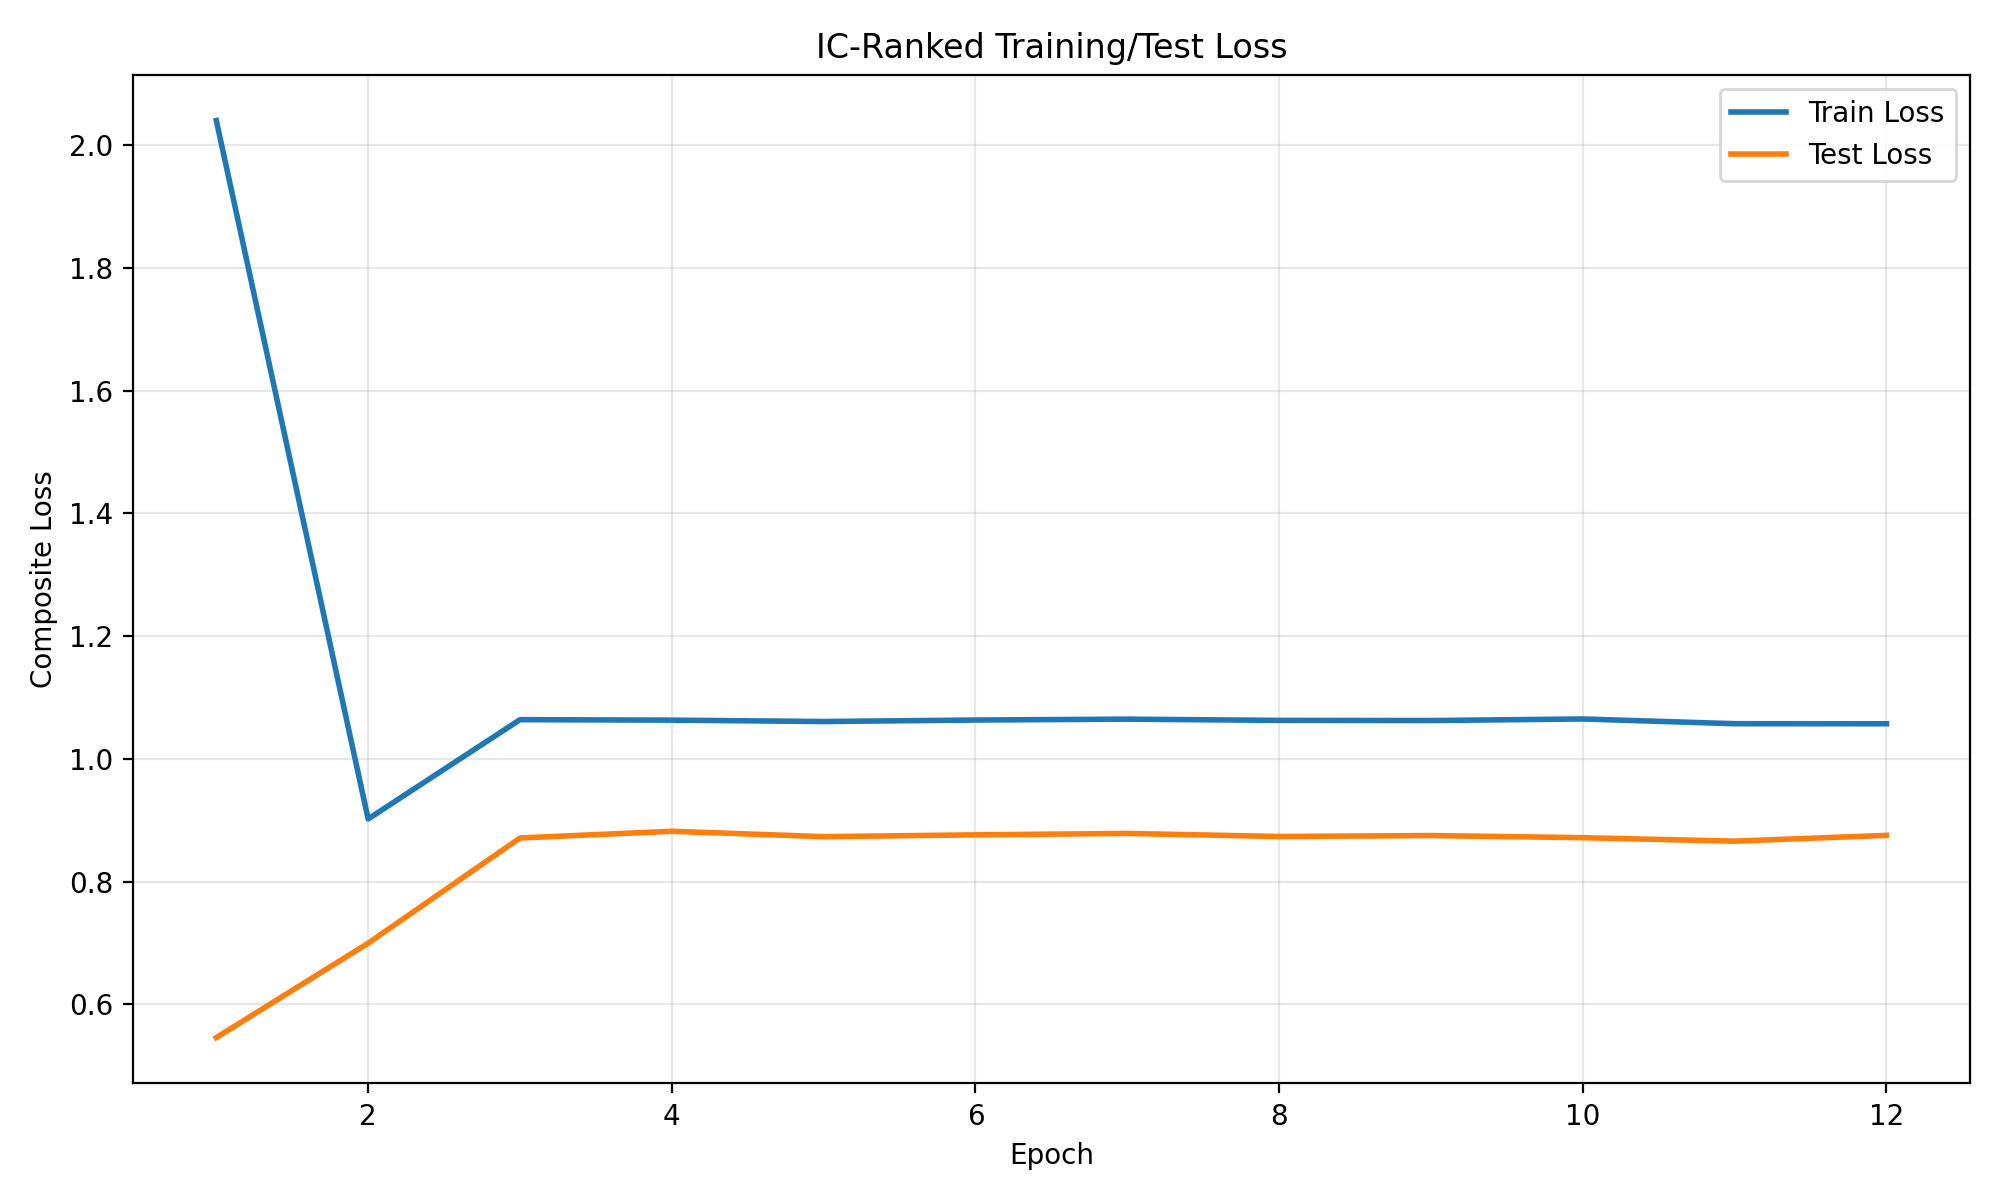
\includegraphics[width=\textwidth]{data/plots/2024-12-31_icrank_loss_curve.png}
      \small Loss curves (MSE + IC + dispersion) across all three splits.
      IC warmup visible in the first 10 epochs.
    \end{column}
  \end{columns}
\end{frame}

\begin{frame}{Live Predictions — March 2026}
  \begin{columns}[T]
    \begin{column}{0.48\textwidth}
      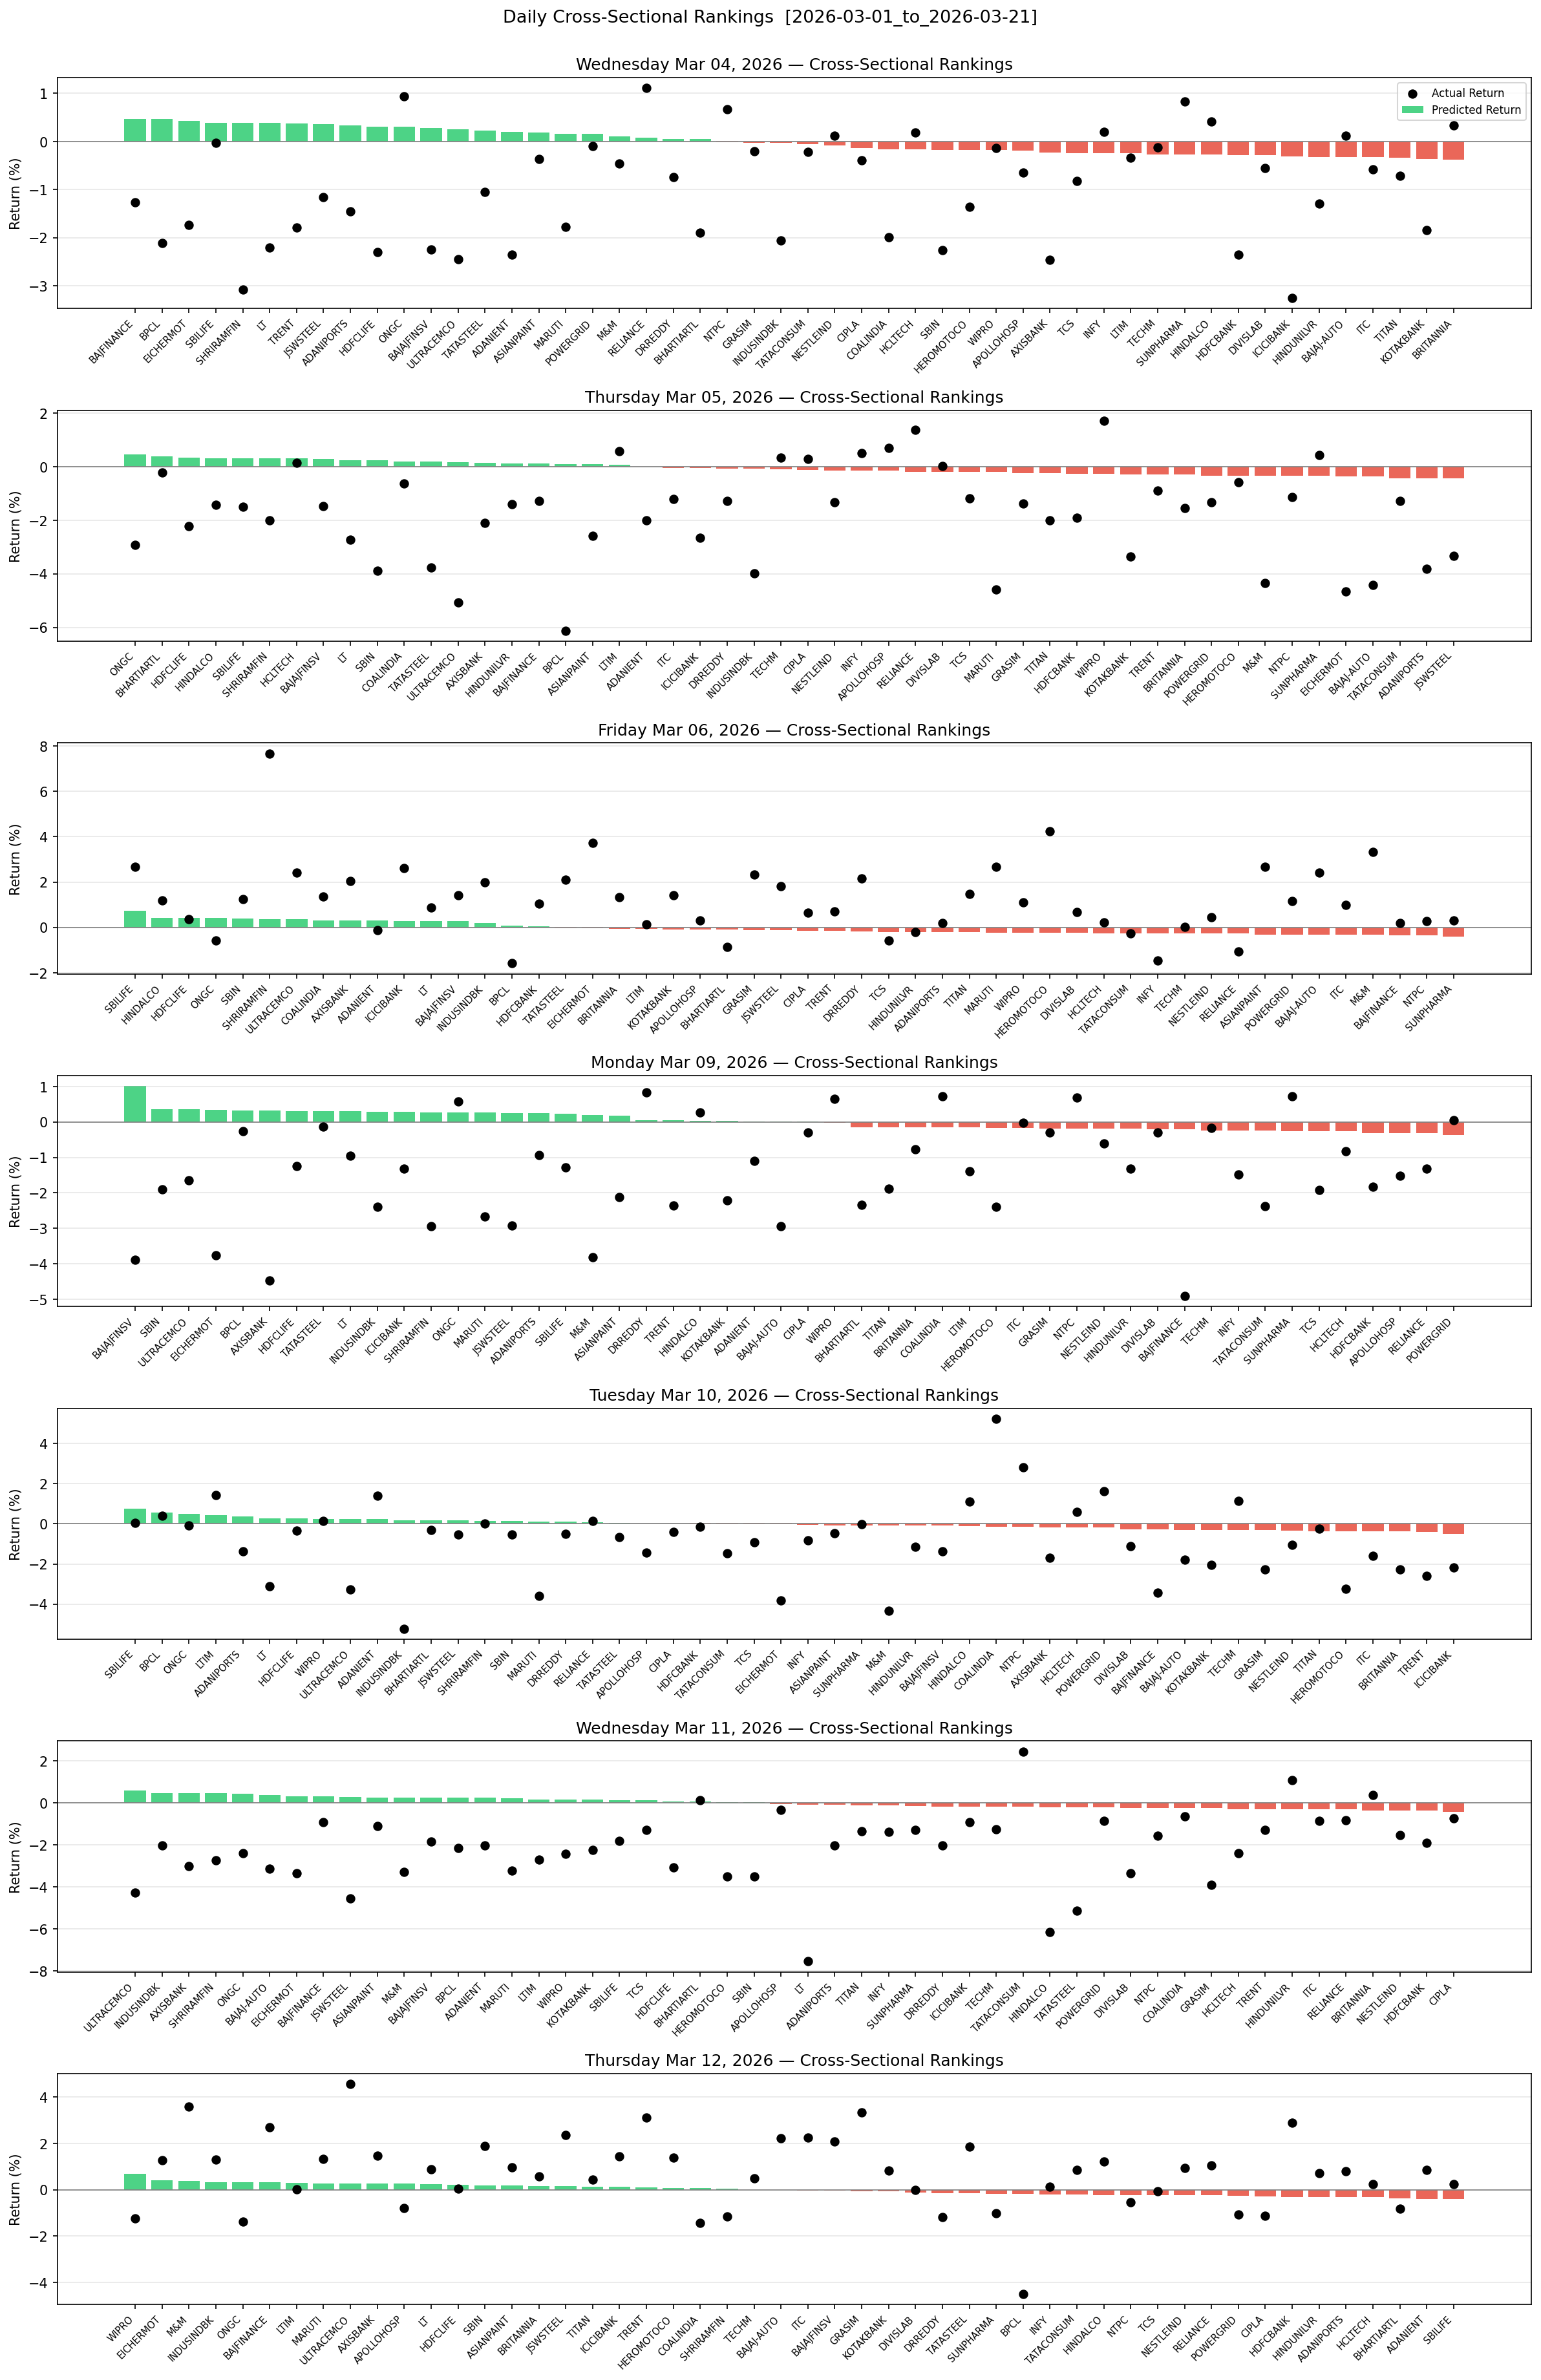
\includegraphics[width=\textwidth]{data/plots/live_rankings_2026-03-01_to_2026-03-21.png}
      \small Predicted daily rankings across all 50 Nifty stocks.
    \end{column}
    \begin{column}{0.48\textwidth}
      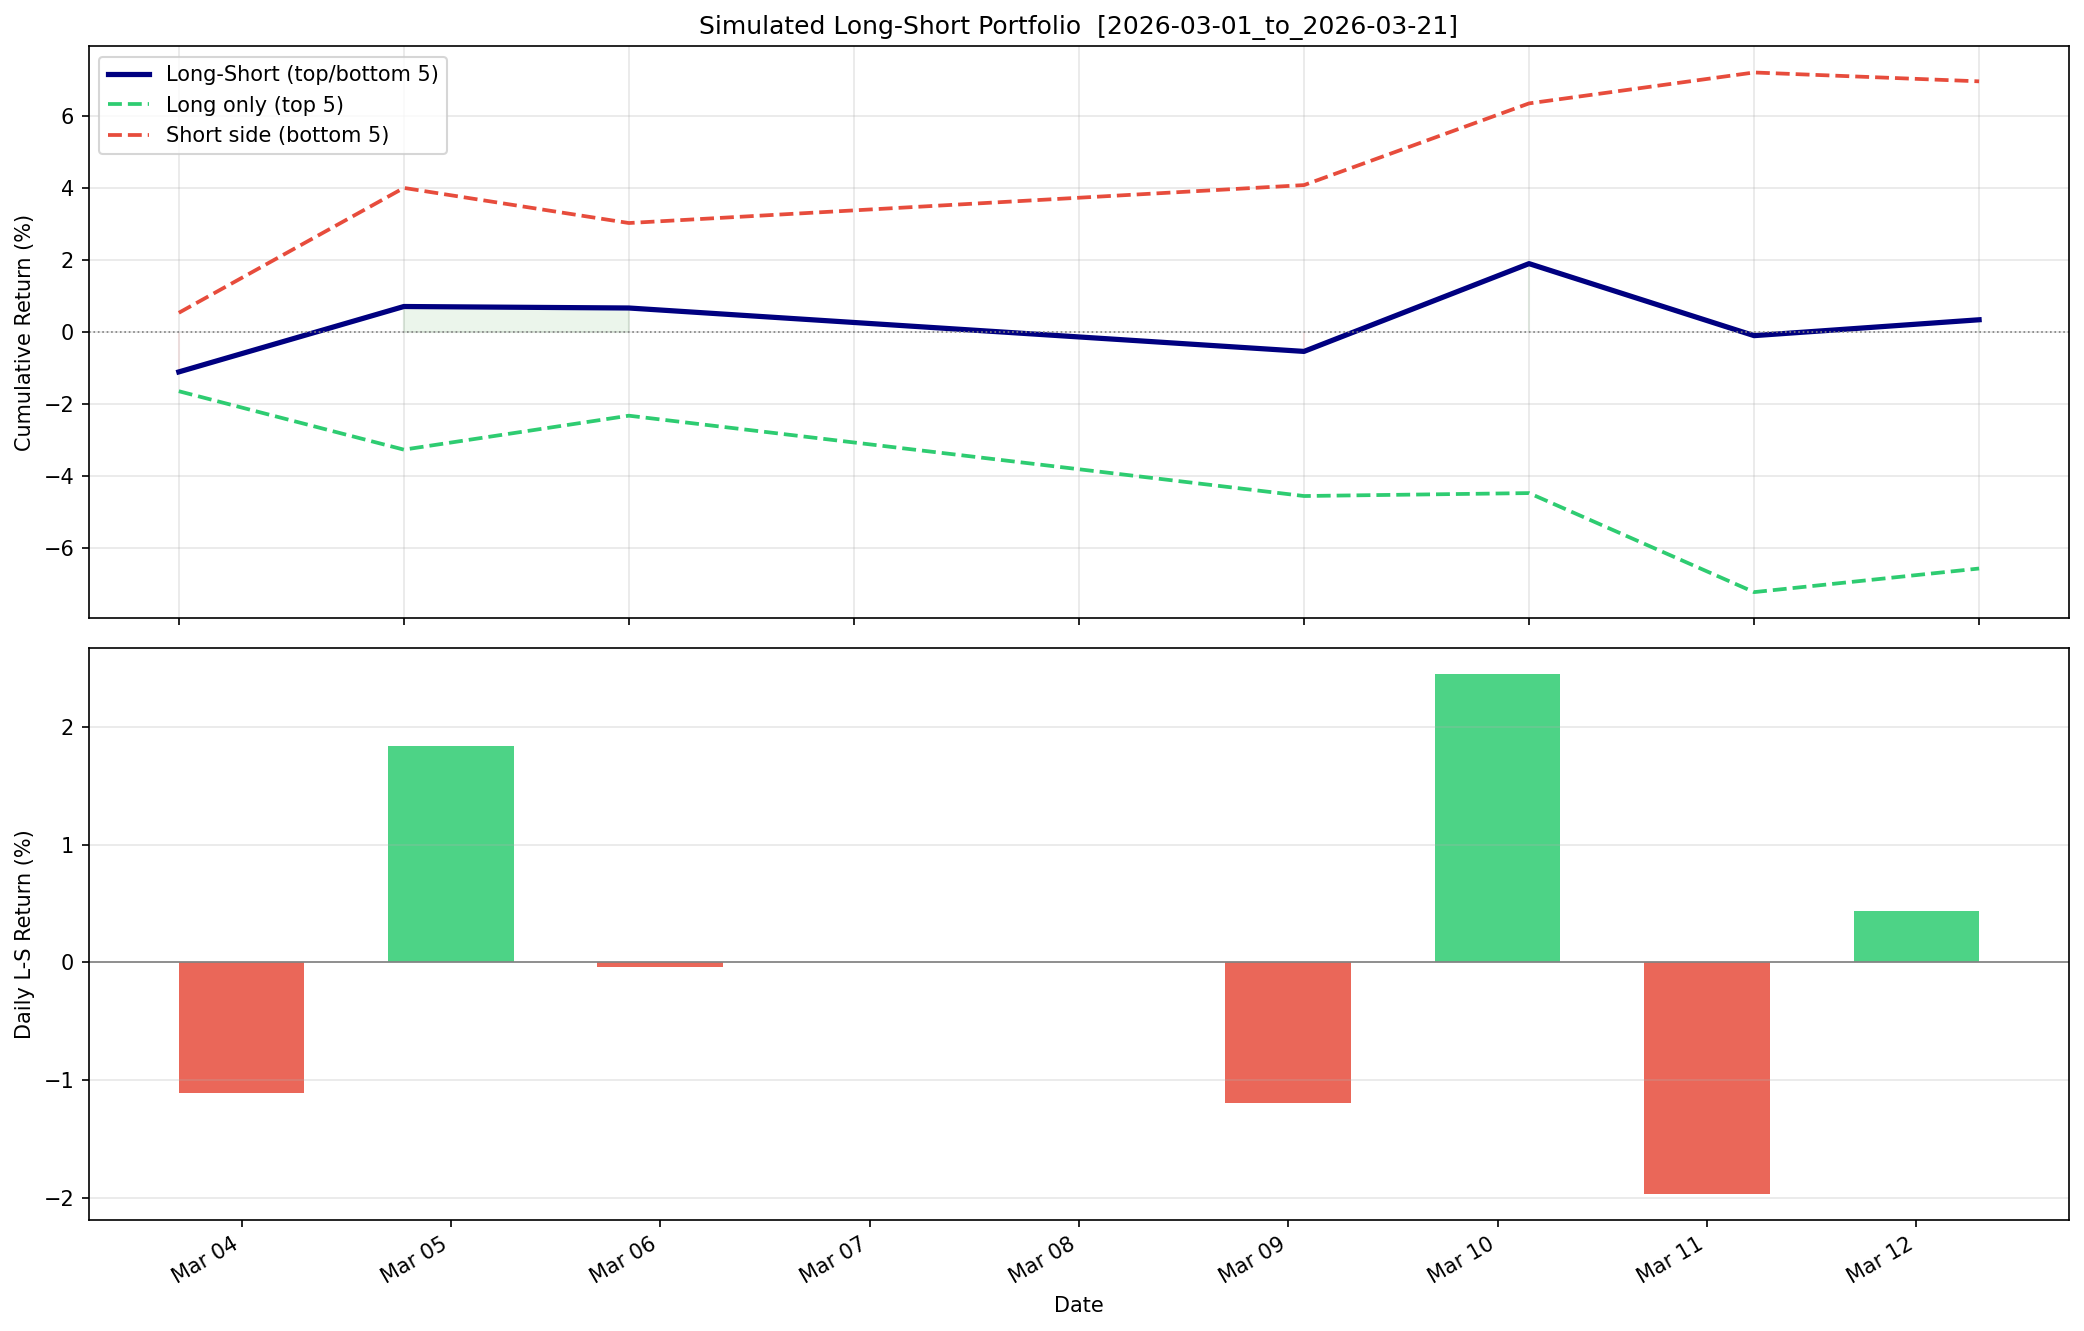
\includegraphics[width=\textwidth]{data/plots/live_longshort_2026-03-01_to_2026-03-21.png}
      \small Long-short portfolio: top-5 minus bottom-5 cumulative return.
    \end{column}
  \end{columns}
\end{frame}

\begin{frame}{Live Predictions — Individual Stocks}
  \begin{columns}[T]
    \begin{column}{0.48\textwidth}
      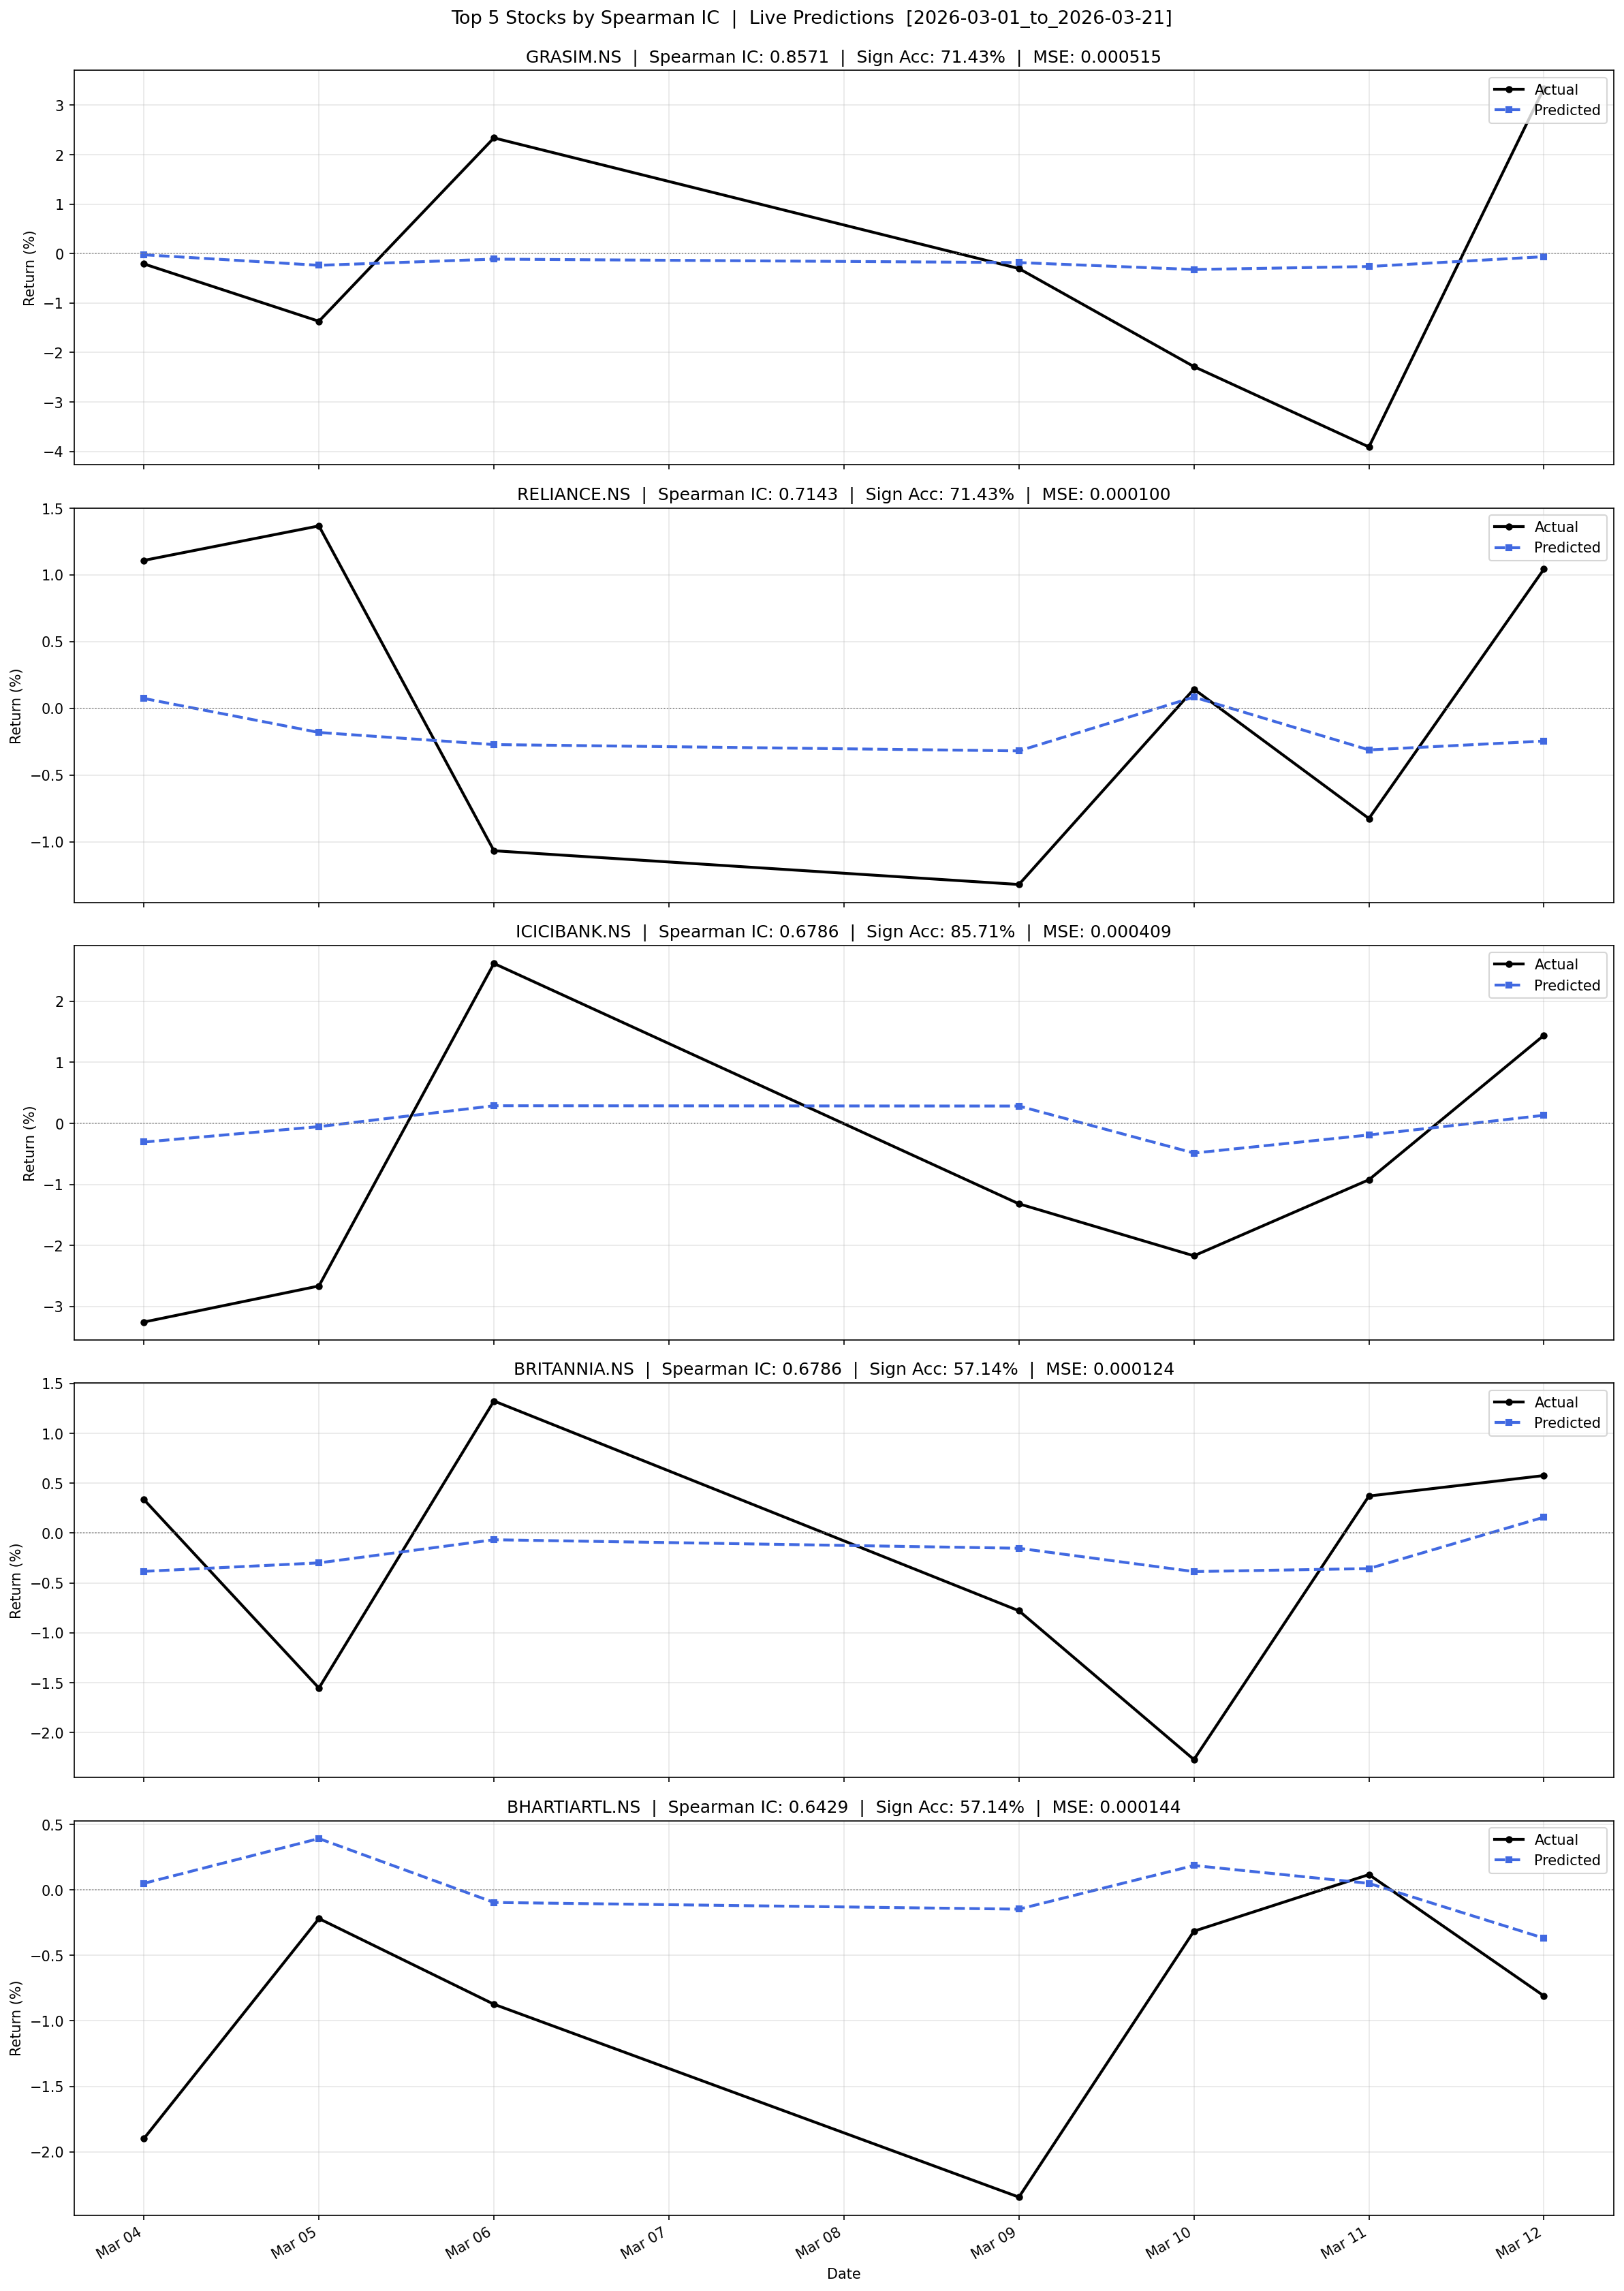
\includegraphics[width=\textwidth]{data/plots/live_top5_2026-03-01_to_2026-03-21.png}
      \small Predicted vs.\ actual returns for top-5 ranked stocks.
    \end{column}
    \begin{column}{0.48\textwidth}
      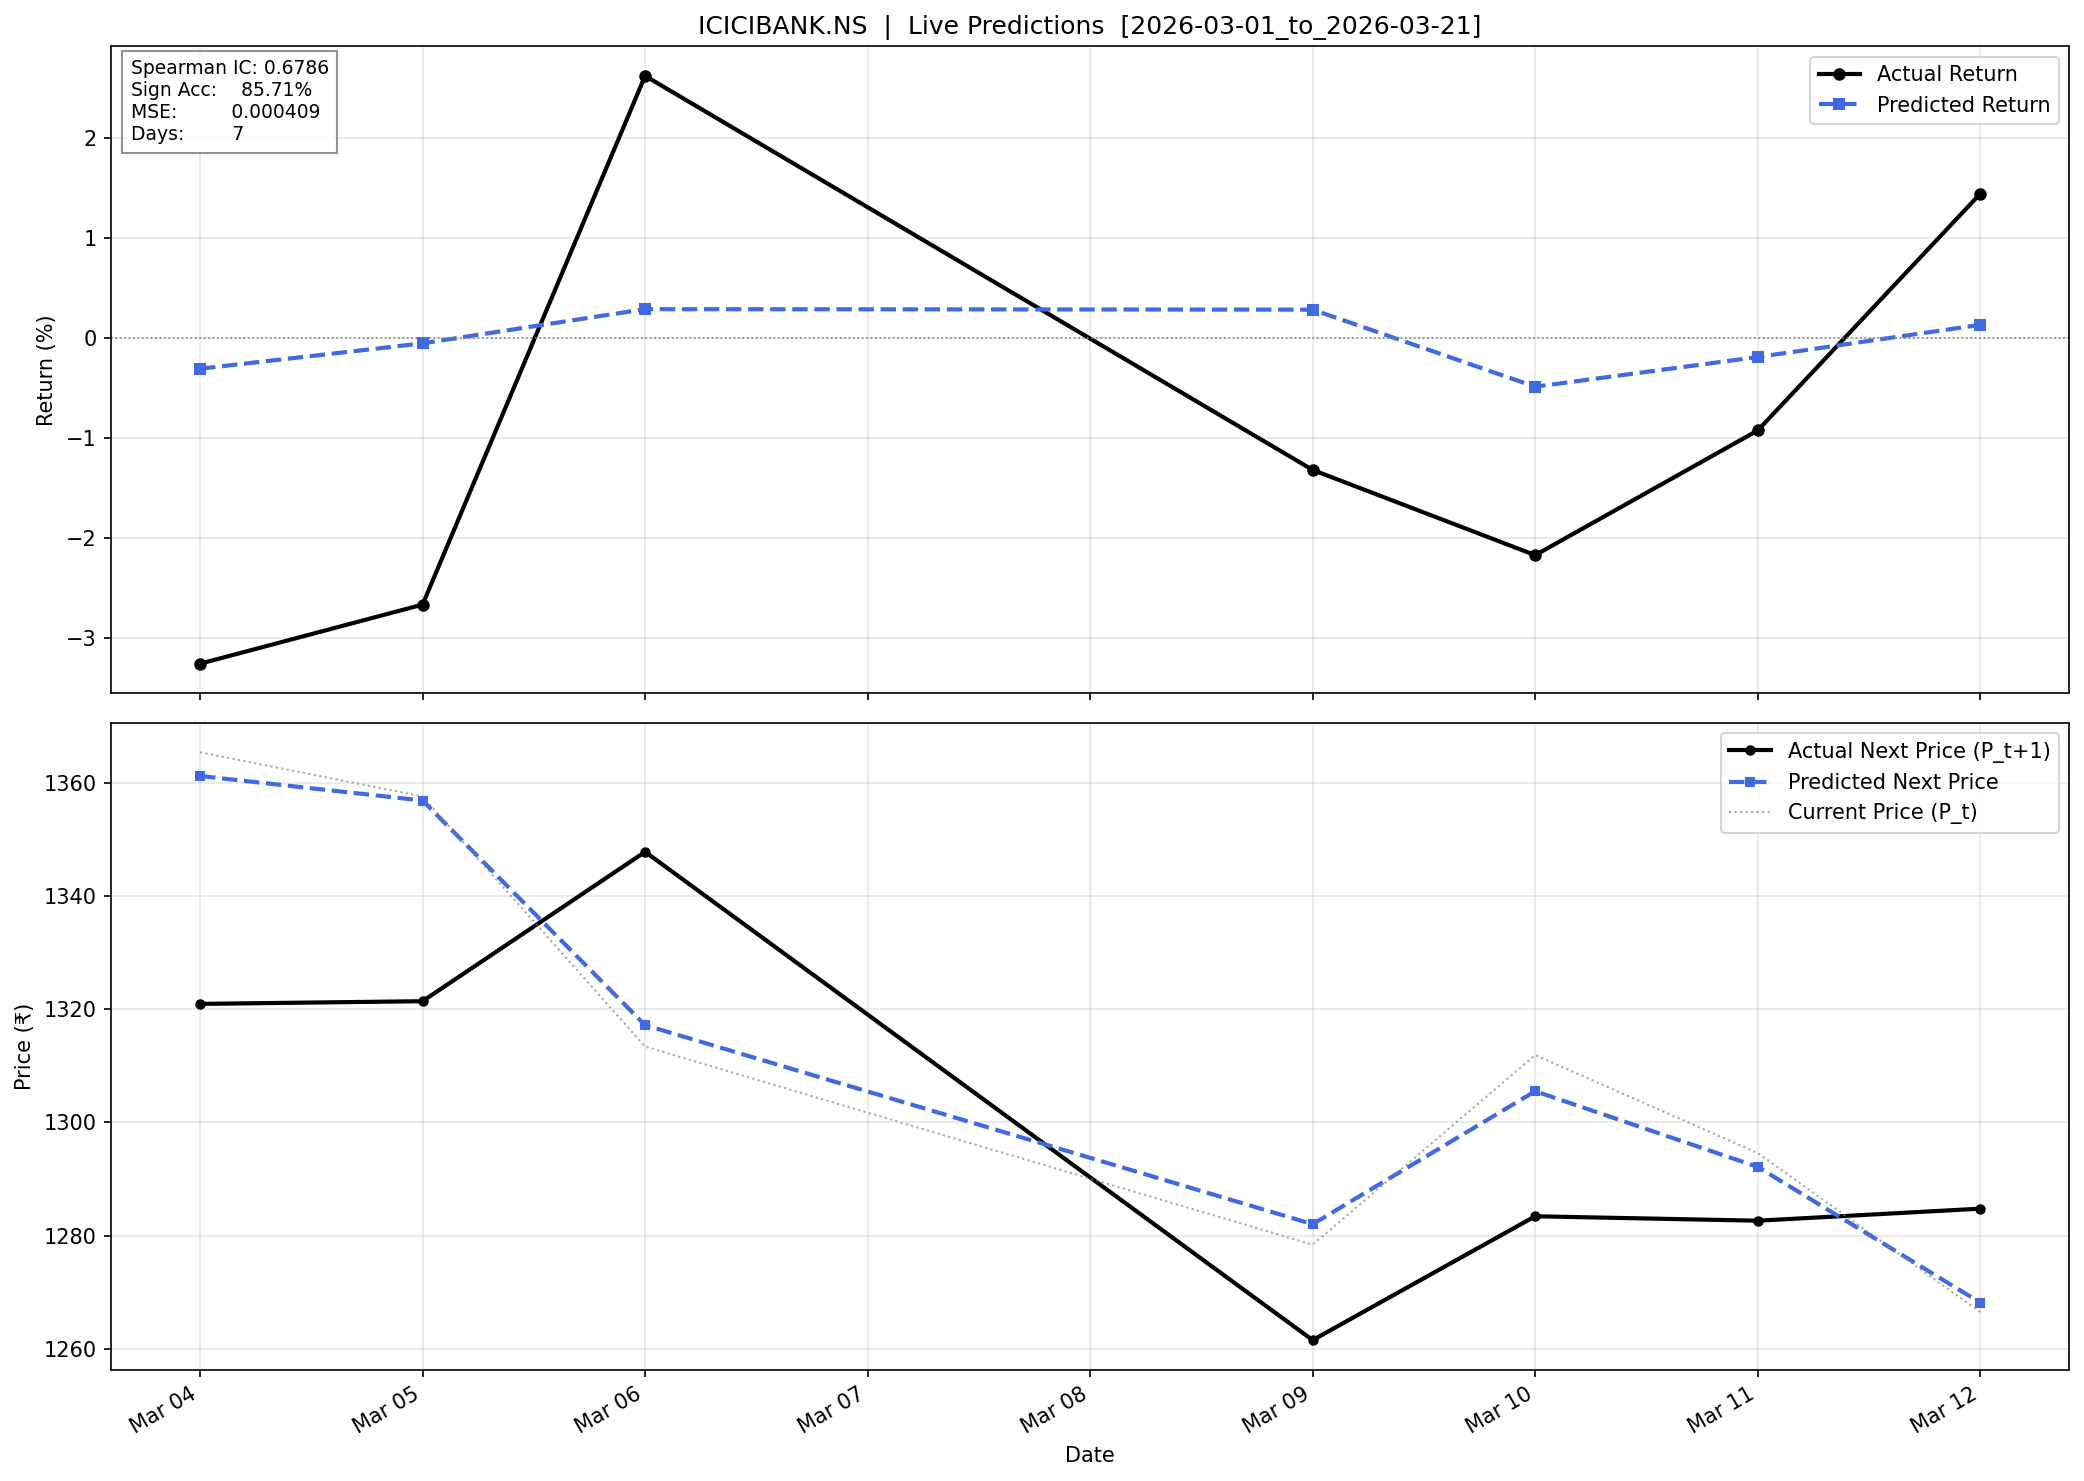
\includegraphics[width=\textwidth]{data/plots/live_2026-03-01_to_2026-03-21_ICICIBANK.NS.png}
      \small ICICIBANK: predicted vs.\ actual next-day return.
    \end{column}
  \end{columns}
\end{frame}

% ============================================================
\section{Limitations \& Future Work}
% ============================================================

\begin{frame}{Current Limitations}
  \begin{columns}[T]
    \begin{column}{0.48\textwidth}
      \textbf{Architecture:}
      \begin{itemize}
        \item \textbf{Pairwise constraint}: THGNN can only model two-stock
              relationships; higher-order group dynamics (sector-wide shocks)
              are decomposed into pairwise edges, losing higher-order signal
        \item \textbf{Static graph topology within a window}: adjacency is
              recomputed daily but remains fixed within a forward pass
        \item \textbf{GRU vs.\ Transformer}: GRU may under-capture long-range
              temporal dependencies compared to attention-based encoders
      \end{itemize}
    \end{column}
    \begin{column}{0.48\textwidth}
      \textbf{Training \& Data:}
      \begin{itemize}
        \item \textbf{Universe size}: limited to 50 stocks (Nifty 50); does
              not generalise across index changes
        \item \textbf{Feature set}: 6 OHLCV features; no macro, sentiment, or
              order-book features
        \item \textbf{Ranking objective}: trained with MSE + soft-IC, not a
              pure profit-maximisation criterion (STHAN-SR addresses this)
        \item \textbf{Transaction costs}: live evaluation ignores slippage and
              market impact
      \end{itemize}
    \end{column}
  \end{columns}
\end{frame}

\begin{frame}{Future Directions — Towards Hypergraph Architectures}
  \begin{columns}[T]
    \begin{column}{0.55\textwidth}
      \textbf{Short-term improvements to THGNN:}
      \begin{enumerate}
        \item Replace GRU with Transformer encoder (patch-based, like StockMixer)
        \item Add macro indicators as \emph{global} node features
        \item Walk-forward re-training with calendar rebalancing
      \end{enumerate}

      \bigskip
      \textbf{Hypergraph extensions:}
      \begin{enumerate}
        \setcounter{enumi}{3}
        \item \textbf{STHAN-SR}: replace regression loss with
              learning-to-rank (ListNet / LambdaRank) directly optimising
              portfolio selection
        \item \textbf{MaGNet}: probabilistic hyperedges with soft stock
              membership across latent market themes
        \item Dynamic hyperedge discovery via spectral clustering on the
              time-varying correlation tensor
      \end{enumerate}
    \end{column}
    \begin{column}{0.42\textwidth}
      \begin{block}{Why Hypergraphs?}
        \begin{itemize}
          \item A single macro event (e.g.\ RBI rate change) affects an
                \emph{entire sector} simultaneously — this is a hyperedge,
                not a collection of pairwise edges
          \item Stocks belong to multiple \emph{overlapping} themes
                (e.g.\ HDFC is both banking and Nifty 50 index constituent)
          \item Group-wise information aggregation is more expressive and
                preserves higher-order market structure
        \end{itemize}
      \end{block}
    \end{column}
  \end{columns}
\end{frame}

% ============================================================
\section{Conclusion}
% ============================================================

\begin{frame}{Conclusion}
  \begin{columns}[T]
    \begin{column}{0.55\textwidth}
      \textbf{Contributions:}
      \begin{itemize}
        \item Full implementation of THGNN on Nifty 50 with dynamic,
              day-specific correlation graphs
        \item Composite IC-ranked loss (MSE + soft Spearman IC + dispersion)
              that aligns training with portfolio ranking objectives
        \item Heterogeneous positive/negative graph attention distinguishes
              fundamentally different market relationship types
        \item Clean three-stage data pipeline reproducible from raw Yahoo
              Finance data
      \end{itemize}
    \end{column}
    \begin{column}{0.42\textwidth}
      \textbf{Key takeaways:}
      \begin{enumerate}
        \item Graph structure consistently improves over independent-stock
              baselines by enabling information flow across correlated stocks
        \item Soft Spearman IC loss is more aligned with portfolio evaluation
              than pure MSE
        \item Pairwise GNNs remain limited — the next frontier is
              \textbf{hypergraph architectures} for group-wise market dynamics
      \end{enumerate}

      \bigskip
      \begin{block}{Best Val IC}
        \centering
        $\text{IC}_\text{val} = 0.029$\\
        \small (trained on 9 years Nifty 50 data)
      \end{block}
    \end{column}
  \end{columns}
\end{frame}

% ---- Appendix -----------------------------------------------
\appendix

\begin{frame}{References}
  \begin{thebibliography}{9}
    \bibitem{thgnn2022}
      Xiang et al.\ (2022).
      \textit{Temporal and Heterogeneous Graph Neural Network for Financial
      Time Series Prediction.}
      CIKM 2022.
      \href{https://doi.org/10.1145/3511808.3557089}{doi:10.1145/3511808.3557089}

    \bibitem{master2023}
      Ma et al.\ (2023).
      \textit{MASTER: Market-Guided Stock Transformer for Stock Price
      Forecasting.}
      AAAI 2024.

    \bibitem{stockmixer2024}
      Zhang et al.\ (2024).
      \textit{StockMixer: A Simple Yet Strong MLP Mixer for Stock
      Price Forecasting.}

    \bibitem{sthan2021}
      Sawhney et al.\ (2021).
      \textit{Stock Selection via Spatiotemporal Hypergraph Attention Network:
      A Learning to Rank Approach.}
      AAAI 2021.

    \bibitem{magnet2022}
      \textit{MaGNet: Multi-scale Graph-Guided Attention Network for Stock
      Prediction.}
      2022.

    \bibitem{pairnorm2020}
      Zhao et al.\ (2020).
      \textit{PairNorm: Tackling Oversmoothing in GNNs.}
      ICLR 2020.
  \end{thebibliography}
\end{frame}

\begin{frame}{Model Hyperparameters — Full Reference}
  \begin{center}
  \renewcommand{\arraystretch}{1.3}
  \begin{tabular}{lll}
    \toprule
    \textbf{Parameter} & \textbf{Default} & \textbf{Description} \\
    \midrule
    \texttt{in\_features}   & 6   & Input channels per timestep \\
    \texttt{hidden\_dim}    & 128 & GRU hidden size + MLP width \\
    \texttt{num\_layers}    & 1   & GRU layers \\
    \texttt{num\_heads}     & 8   & GAT attention heads \\
    \texttt{out\_features}  & 32  & Per-head GAT output dim \\
    \texttt{dropout}        & 0.3 & Applied after GRU and each MLP \\
    \midrule
    \texttt{mse\_weight}        & 1.0  & Weight on normalised MSE \\
    \texttt{ic\_weight}         & 0.35 & Weight on IC ranking loss \\
    \texttt{dispersion\_weight} & 0.2  & Weight on spread-ratio penalty \\
    \texttt{return\_scale}      & 0.01 & MSE normalisation constant \\
    \texttt{ic\_warmup\_epochs} & 10   & IC ramp-up duration \\
    \midrule
    \texttt{lr}           & $10^{-4}$ & AdamW learning rate \\
    \texttt{weight\_decay}& $10^{-3}$ & L2 regularisation \\
    \texttt{patience}     & 20        & Early stopping \\
    \texttt{epochs}       & 60        & Maximum epochs \\
    \bottomrule
  \end{tabular}
  \end{center}
\end{frame}

\end{document}
